\documentclass[12pt,letterpaper]{article}
%%%%%%%%%%%%%%%%% common packages are included here %%%%%%%%%%%%%%%%%
\usepackage{graphicx}
\usepackage{epstopdf}
\usepackage{tabularx}
\usepackage[lofdepth,lotdepth]{subfig} % subfloat
\usepackage{bm} % bold math
\usepackage{color}
\usepackage[centertags]{amsmath}
\usepackage{mathrsfs}
\usepackage{amsmath}
\usepackage{mathtools}
\usepackage{amssymb}
\usepackage{amsfonts}
\usepackage{amssymb}
\usepackage{amsthm}
\usepackage{newlfont}
\usepackage{textcomp,gensymb} % for \textcelsius, \textdegree, and \degree
\usepackage{syntonly}

%%%%%%%%%%%%%%%%%%%% some declaration %%%%%%%%%%%%%%%%%%%%%
\DeclareGraphicsExtensions{.pdf,.png,.jpg,.eps}
\graphicspath{{./figures/}}

%%%%%%%%%%%%%%%%%%% new commands are defined here %%%%%%%%%%%%%%%%%%%%%
\newcommand{\dg}{$^{\circ}$} % degree symbol
\newcommand{\iang}{\AA$^{-1}$} % inverse Angstrom symbol
\newcommand{\degC}{$^{\circ}\mathrm{C}$} % degree Celcius
\newcommand{\Eq}[1]{Eq.\,(\ref{#1})} % reference to an equation

% Some mathematical (physical) quantities and symbols that are used often
\newcommand{\xhat}{\mathbf{\hat{x}}}
\newcommand{\yhat}{\mathbf{\hat{y}}}
\newcommand{\zhat}{\mathbf{\hat{z}}}
\newcommand{\kin}{\mathbf{k}_{\mathrm{in}}}
\newcommand{\kout}{\mathbf{k}_{\mathrm{out}}}
\newcommand{\Tat}{\mathrm{Tat}}
\newcommand{\DOPC}{\mathrm{DOPC}}
\newcommand{\cm}{\mathrm{cm}}

% To simplify some formatting issues
\newcommand{\pars}[1]{\mathopen{}\left( #1 \right)\mathclose{}} % () without extra spaces due to \left and \right
\newcommand{\angles}[1]{\left\lange #1 \right\rangle}%      <>
\newcommand{\braces}[1]{\left\lbrace #1 \right\rbrace}%     {}
\newcommand{\bracks}[1]{\left\lbrack #1 \right\rbrack}%     []
\newcommand{\ds}[1]{\displaystyle{#1}}%
\newcommand{\+}{^{\dagger}}%                                
\newcommand{\partiald}[3][]{{\partial^{#1}#2 \over \partial {#3}^{#1}}}%


\newcommand{\dx}{\mathop{dx}}
\newcommand{\dy}{\mathop{dy}}
\newcommand{\dz}{\mathop{dz}}

\newcommand{\FC}{F_\mathrm{C}}
\newcommand{\FT}{F_\mathrm{T}}
% Z's
\newcommand{\zh}[1]{Z_{\mathrm{H}#1}}
\newcommand{\zw}{Z_\mathrm{W}}
\newcommand{\zchtwo}{Z_\mathrm{CH_2}}
% sigma's
\newcommand{\sigmah}[1]{\sigma_{\mathrm{H}#1}}
\newcommand{\sigmam}{\sigma_\mathrm{M}}
% rho's
\newcommand{\rhoh}[1]{\rho_{\mathrm{H}#1}}
\newcommand{\rhom}{\rho_\mathrm{M}}
\newcommand{\rhog}{\rho_\mathrm{G}}
\newcommand{\rhos}{\rho_\mathrm{S}}
\newcommand{\rhob}{\rho_\mathrm{B}}
\newcommand{\rhow}{\rho_\mathrm{W}}
\newcommand{\rhochtwo}{\rho_\mathrm{CH_2}}
\newcommand{\deltazh}{\Delta Z_\mathrm{H}}
\newcommand{\Rhm}[1]{R_{\mathrm{H}#1\mathrm{M}}}
% subscript
\newcommand{\chtwo}{\mathrm{CH_2}}
\newcommand{\w}{\mathrm{W}}

%\syntaxonly
\usepackage[pdftex]{hyperref}
\usepackage{graphicx}

%%%%%%%%%%%%%%%%%%%%%%%%%%%%%%%%%%%%%%%%%%%%%%%%%%%%%%%%%%%%%%%%%%%%%%%%%%%%%%%
\begin{document} %%%%%%%%%%%%%%%%%%%%%%%%%%%%%%%%%%%%%%%%%%%%%%%%%%%%%%%%%%%%%%
\today %%%%%%%%%%%%%%%%%%%%%%%%%%%%%%%%%%%%%%%%%%%%%%%%%%%%%%%%%%%%%%%%%%%%%%%%
%%%%%%%%%%%%%%%%%%%%%%%%%%%%%%%%%%%%%%%%%%%%%%%%%%%%%%%%%%%%%%%%%%%%%%%%%%%%%%%
\section{Scattering Basics}
The incoming and outgoing wavevectors of the x-ray beam in Fig. XXX 
are given by
\begin{equation}
  \kin = \frac{2\pi}{\lambda} \yhat, \quad
  \kout = 
    \frac{2\pi}{\lambda} \left( 
      \sin 2\theta \cos\phi \, \xhat
      + \cos 2\theta \, \yhat
      + \sin 2\theta \sin\phi \, \zhat 
    \right),
  %\label{eq:kinkout}
\end{equation}
where $\lambda$ is the wavelength of x-ray, $2\theta$ is the total scattering
angle, and $\phi$ is the angle measured from the equator on the detector. 
The scattering vector (also called
momentum transfer vector) is
the difference between $\kin$ and $\kout$,
\begin{align}
  \mathbf{q} &= \kout - \kin \nonumber \\
             &= q \left( 
                  \cos\theta\cos\phi \, \xhat - \sin\theta \, \yhat
                  + \cos\theta\sin\phi \, \zhat
                \right),
  \label{eq:q_vector}
\end{align}
where $q=4\pi\sin\theta/\lambda$ is the magnitude of the scattering vector. 
When the sample is rotated by $\omega$ about the lab x-axis in the clockwise 
direction as shown in Fig. XXX, the sample coordinates differ from the lab 
coordinates and are given by  
\begin{equation}
  \mathbf{\hat{e}_x} = \xhat, \quad
  \mathbf{\hat{e}_y} = \cos\omega\,\yhat + \sin\omega\,\zhat, \quad
  \mathbf{\hat{e}_z} = -\sin\omega\,\yhat + \cos\omega\,\zhat.
  \label{eq:smp_coord}
\end{equation}
From Eq.~(\ref{eq:q_vector}) and (\ref{eq:smp_coord}), we find the projection of 
$\mathbf{q}$ on the sample coordinates to be
\begin{align}
  q_x &= \mathbf{q}\cdot\mathbf{\hat{e}_x} 
       = q\cos\theta\cos\phi, 
       \nonumber\\
  q_y &= \mathbf{q}\cdot\mathbf{\hat{e}_y} 
       = q\left(-\sin\theta\cos\omega + \cos\theta\sin\phi\sin\omega\right), 
       \nonumber\\
  q_z &= \mathbf{q}\cdot\mathbf{\hat{e}_z} 
       = q\left(\sin\theta\sin\omega + \cos\theta\sin\phi\cos\omega\right).
       \label{eq:qxqyqz}
\end{align}
The position, $(X,Z)$, of a CCD pixel is measured with respect to the beam 
and given by
\begin{equation}
  X = S \tan 2\theta \cos\phi, \quad Z = S \tan 2\theta \sin\phi,
  \label{eq:XZ}
\end{equation} 
where $S$ is the distance between the sample and detector.
From a model for the electron density of a lipid bilayer, one calculates
a X-ray scattering intensity pattern, $I(\mathbf{q})$. Then, Eq.~(\ref{eq:qxqyqz})
and (\ref{eq:XZ}) relate $I(\mathbf{q})$ to the experimentally measured
intensity pattern, $I(X,Z)$. It is important to remember that a given pixel
position, $(X,Z)$, corresponds to a triplet $(q_x, q_y, q_z)$. Fully exploring 
the sample $q$-space requires changing $\omega$ for a fixed wavelength, which was
achieved by continuously rotating the sample with a motor. In the ripple phase, 
because our sample has in-plane rotational symmetry,
the ripple side peaks make up Bragg rings while the main peaks are still 
delta function like (see Fig. X) in $q$-space. In order for the main peak to be
observed, $\omega$ must be equal to $\theta_\mathrm{B}$, but the side peaks
are observed at any $\omega$. Those side peaks get slightly smeared due to 
integration over $q_y$.

For low angle x-ray scattering (LAXS), it is convenient to linearlize the above
equations in terms of $\theta$ and $\omega$. In the small angle approximation, 
$\sin\phi \approx Z/(2S\theta)$ and $\cos\phi \approx X/(2S\theta)$, and
\begin{align}
  q_x &\approx \frac{4\pi\theta\cos\phi}{\lambda} \approx kX/S \nonumber\\
  q_y &\approx q_z\omega -\frac{4\pi\theta^2}{\lambda} \approx q_z\omega - \frac{\lambda q_z^2}{4\pi}\nonumber\\
  q_z &\approx \frac{4\pi\theta\sin\phi}{\lambda} \approx kZ/S,
  \label{eq:qxqyqz_small}
\end{align}
with $k=2\pi/\lambda$. For wide angle X-ray scattering, the exact relations given
by Eq.~(\ref{eq:qxqyqz}) are necessary. Especially in the transmission experiment,
where $\omega$ is large, an observed X-ray pattern appears nontrivial and becomes
almost impossible to analyze without the use of Eq.~(\ref{eq:qxqyqz}).


%%%%%%%%%%%%%%%%%%%%%%%%%%%%%%%%%%%%%%%%%%%%%%%%%%%%%%%%%%%%%%%%%%%%%%%%%%%%%%%
\section{Geometric Correction for the Ripple Phase Scattering}
In order to capture both main and side peaks in one x-ray exposure, 
the sample was continuously rotated. As a result of the rotation, 
the main peaks become arcs that subtend an angle $2\theta_{h}$ ,
as shown in Fig.~\ref{fig:ewald_main}, with its length
equal to $2\theta_{h}q_{z,h}$.  
%----------------------------------------------
\begin{figure}[htbp]
  \centering
  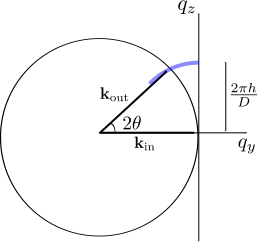
\includegraphics[scale=1]{figures/ewald_main}
  \caption{caption goes here}
  \label{fig:ewald_main}
\end{figure}
%----------------------------------------------
What is recorded on the detector is the cross section of this arc with the 
Ewald sphere, so the total intensity is the product of the observed intensity
with the arc length, that is, 
\begin{equation}
  I = 2\theta_{h}q_{z,h} I_{\mathrm{o},h}. \label{eq:main_ewald}
\end{equation}

Because the sample has in-plane rotational symmetry, the side peaks turn
into Bragg rings whose radius is $q_{r,k}$, as shown in Figure X. 
These rings cross the Ewald sphere
at all angles of $\omega$. Then, the total intensity is given by
\begin{equation}
  I=2\pi q_{r,k} I_{\mathrm{o},k}. \label{eq:side_ewald}
\end{equation}
Inverting Eq.~(\ref{eq:main_ewald}) and (\ref{eq:side_ewald}) 
and realizing that the intensity is the form factor
squared, we can calculate the observed intensity, $I_\mathrm{o}$, 
from a model for electron density in the ripple phase.

Mathematically, the rotation is  
equivalent to an integration over $\omega$. In low angle X-ray scattering, 
$q_z$ is constant at a given pixel as $\omega$ is changed, which can be seen from 
Eq.~(\ref{eq:qxqyqz_small}). $\omega$ dependence appears only through $q_y$, 
so rotating the sample is realized by integrating over $q_y$. 
To derive the integration limits, let us consider two cases: (a) When $\omega \leq 0$,
the incoming X-ray beam is blocked by the back of the substrate. This sets 
the lower limit to 0. (b) When $\omega \geq 2\theta$, the substrate blocks 
the outgoing X-ray. Within the small angle approximation, then, $\omega_{\text{max}}$
is $2\times \lambda q_z/(4\pi)$. Thus, the integration limits 
for $q_y$ integration are $[-\lambda q_z^2/(4\pi), \lambda q_z^2/(4\pi)]$.
We also need to integrate over $X$ and $Z$ to obtain integrated intensity. 
These lead to the observed intensity
written as,
\begin{align}
  I_{\mathrm{o},hk} 
    &\propto \int dX \int dZ \int d\omega |F_{hk}|^2 S_{hk}(\mathbf{q}) \nonumber \\
    &\propto |F_{hk}|^2 \int dq_x \int dq_z 
             \int_{-\frac{\lambda q_z^2}{4\pi}}^{\frac{\lambda q_z^2}{4\pi}} \frac{dq_y}{q_z} 
             S_{hk}(\mathbf{q}),
\end{align}
where $1/q_z$ factor in $q_y$ integration is the Lorentz polarization factor
in the small angle approximation. 

For a crystalline sample with the in-plane rotational symmetry, the
structure factor is  
\begin{equation}
  S_{hk}(\mathbf{q}) = S_{hk}(q_r,q_z) 
  = \frac{1}{2\pi q_r}\delta(q_r-q_{r,k})\delta(q_z-q_{z,hk}),
\end{equation} 
where $q_{r,k}=2\pi |k|/\lambda_r$. Thus, the scattering pattern in the 
ripple phase is a 
collection of Bragg ``rings'' centered at the meridian and the 
Bragg peaks that are called the main peaks.  

The observed, integrated intensity of $hk$ peak is proportional to
\begin{equation}
  I_{\mathrm{o},hk} 
    \propto \frac{\lvert F_{hk} \rvert^2}{q_{z,hk}} \int\mathop{dq_x} 
            \int_{-q_{y0}}^{q_{y0}}
            \mathop{dq_y} \frac{\delta(q_r-q_{r,k})}{2\pi q_r},
\end{equation}
where $q_{y0} = \lambda q_{z,hk}^2/(4\pi)$.
For side peaks ($k \neq 0$), we have 
\begin{align}
  \int\mathop{dq_x} \int_{-q_{y0}}^{q_{y0}}\mathop{dq_y} \frac{\delta(q_r-q_{r,k})}{2\pi q_r}
  &\approx \int_{-\frac{q_{y0}}{q_{r,k}}}^{\frac{q_{y0}}{q_{r,k}}} \mathop{d\phi} 
          \int \mathop{dq_r} q_r\frac{\delta(q_r-q_{r,k})}{2\pi q_r} \nonumber\\
 &= \frac{q_{y0}}{\pi q_{r,k}}.
\end{align}
For the main peaks ($k=0$), we have 
\begin{align}
  \int\mathop{dq_x} \int_{-q_{y0}}^{q_{y0}}\mathop{dq_y} \frac{\delta(q_r-q_{r,k})}{2\pi q_r}
  &= \int_0^{2\pi}\mathop{d\phi} \int\mathop{dq_r} q_r\frac{\delta(q_r-q_{r,k})}{2\pi q_r} \nonumber\\
  &= 1
\end{align}
Using Eq.~() and (), we write the observed integrated intensity as
\begin{align}
  I_{\mathrm{o},h0} &\propto \frac{|F_{h0}|^2}{q_{z,h0}} \label{eq:main}\\
  I_{\mathrm{o},hk} &\propto \frac{|F_{hk}|^2}{q_{z,hk}} \frac{q_{y0}}{\pi q_{r,k}}
    = |F_{hk}|^2 \frac{\lambda q_{z,hk}}{2\pi}\frac{1}{2\pi q_{r,k}}
    = |F_{hk}|^2 \frac{2\theta_{hk}}{2\pi q_{r,k}}, \label{eq:side}
\end{align}
where $2\theta_{hk} = \lambda q_{z,hk}/(2\pi)$ is the incident angle at which 
the outgoing x-ray with its scattering angle equal to $\theta_{hk}$ gets 
blocked by the substrate.
Eq.~(\ref{eq:main}) and (\ref{eq:side}) relate the form factor calculated from
a model to the experimentally observed intensity, and are 
equivalent to Eq.~(\ref{eq:main_ewald}) and (\ref{eq:side_ewald}), 
which were derived by using the Ewald sphere. 

In non linear least
square fitting procedure, we fitted the observed integrated intensity to
the calculated intensity from a bilayer model using these geometrical corrections. 
This is mainly due to our ability to determine the experimental uncertainties
on observed intensity rather than the geometrically corrected form factor. 
Fitting observed intensity is simpler because it allows us to avoid 
propagating the uncertainties. 

%%%%%%%%%%%%%%%%%%%%%%%%%%%%%%%%%%%%%%%%%%%%%%%%%%%%%%%%%%%%%%%%%%%%%%%%%%%%%%%
\section{Sawtooth model}
The unit cell vectors in the ripple phase can be expressed as 
\begin{equation}
  \mathbf{a} = \frac{D}{\tan\gamma}\xhat + D\zhat
\end{equation}
and
\begin{equation}
  \mathbf{b} = \lambda_r\xhat.
\end{equation}
The corresponding reciprocal lattice unit cell vectors are given by
\begin{equation}
  \mathbf{A} = \frac{2\pi}{D}\zhat
\end{equation}
and
\begin{equation}
  \mathbf{B} = \frac{2\pi}{\lambda_r}\xhat - \frac{2\pi}{\lambda_r\tan\gamma}\zhat.
\end{equation}
The reciprocal lattice vector, $\mathbf{q}_{hk}$ for the Bragg peak with 
Miller indices $(h,k)$ is 
\begin{equation}
  \mathbf{q}_{hk}=h\mathbf{A}+k\mathbf{B},
\end{equation}
so its components can be written as
\begin{equation}
  q_{x,k} = \frac{2\pi k}{\lambda_r}
\end{equation}
\begin{equation}
  q_y = 0
\end{equation}
\begin{equation}
  q_{z,hk} = \frac{2\pi h}{D} - \frac{2\pi k}{\lambda_r\tan\gamma}
\end{equation}


%%%%%%%%%%%%%%%%%%%%%%%%%%%%%%%%%%%%%%%%%%%%%%%%%%%%%%%%%%%%%%%%%%%%%%%%%%%%%%%
\section{Data}
Figure shows a LAXS pattern from DMPC at 18 \degC. $D=57.9$ \AA. Low
resolution experiment. Up to $h=9$ orders were observed in this
data set. Because of a non-negligible degree of mosaicity in the sample,
strong orders cast their arcs over weaker orders. A care must be 
taken to decompose the intensity at a given pixel to intensity due to
a strong order's arc and to that due to a weak peak. This was achieved
by taking a $q_z$ swath and fitting the intensity to two Gaussian
functions whose widths were determined from the known instrumental 
resolution. Figure shows an example of this operation. Table and
Table show with and without the decomposition operation, respectively. 
For many of the orders observed, errors one would expect from 
neglecting the mosaicity effect were small. For higher orders, however,
this was crucial to obtain the correct integrated intensity.

In order to test the decomposition effect, fits were also performed
for the sum of intensity for orders that overlap. 

First, we fitted the data using only up to $h=3$ orders. What did we get?
How did each model do? Any inconsistency with Sun PNAS?

Next, we fitted every peak we observed. Which model failed?


%%%%%%%%%%%%%%%%%%%%%%%%%%%%%%%%%%%%%%%%%%%%%%%%%%%%%%%%%%%%%%%%%%%%%%%%%%%%%%%
\section{Contour Part of the Form Factor}
As in ref, we take the ripple profile to have a sawtooth-like profile. Its
amplitude is  $A/2$ and the projection of the major arm on the 
ripple direction is $x_0$ as shown in Fig. X. Then, we write the ripple 
profile as
\begin{equation}
  u(x) = \left\{
    \begin{array}{ccc}
    -\frac{A}{\lambda_r-x_0}\left(x+\frac{\lambda_r}{2}\right) 
      & \text{for} 
      & -\frac{\lambda_r}{2} \leq x < -\frac{x_0}{2}, \\
    \frac{A}{x_0}x 
      & \text{for} 
      & -\frac{x_0}{2} \leq x \leq \frac{x_0}{2}, \\
    -\frac{A}{\lambda_r-x_0} \left(x-\frac{\lambda_r}{2}\right)
      & \text{for} 
      & \frac{x_0}{2} < x \leq \frac{\lambda_r}{2}.
    \end{array} \right.
\end{equation}
The ripple profile has the inversion symmetry, so that the resulting
form factor is real. $A$ and $x_0$ are fitting parameters that depend 
on the integrated intensity of each peak while $D$ and $\lambda_r$ are
determined from measuring the positions of the Bragg peaks.

In order to allow the electron density along the ripple direction to 
modulate, we include two additional parameters, one to allow for the electron
density across the minor side to be different by a ratio $f_1$ from the 
electron density across the major side and a second parameter $f_2$, which
is multiplied by $\delta$ functions $\delta(x \pm x_0/2)$ to allow for 
a different electron density near the kink between the major and the minor
sides. 


%%%%%%%%%%%%%%%%%%%%%%%%%%%%%%%%%%%%%%%%%%%%%%%%%%%%%%%%%%%%%%%%%%%%%%%%%%%%%%%
\section{Delta Function Model}


%%%%%%%%%%%%%%%%%%%%%%%%%%%%%%%%%%%%%%%%%%%%%%%%%%%%%%%%%%%%%%%%%%%%%%%%%%%%%%%
\section{2G Hybrid Model}
In the hybrid model, the terminal methyl region of the bilayer is represented
as a Gaussian function \cite{ref:Wiener89}. The headgroups are represented by one 
and two Gaussian
functions in 1G and 2G hybrid model, respectively. The methylene and water 
regions are each treated as a constant. The gap between the two constants is 
represented by a sine function. Then, for half of the bilayer, 
$0 \leq z \leq D/2$, the electron density has the form, 
\begin{equation}
  \rho(z) = \rhog(z) + \rhos(z) + \rhob(z),
\end{equation}
where the Gaussian part is given by 
\begin{equation}
  \rhog(z) = \sum_{i=1}^{1\text{ or }2} \rhoh{i}
             e^{-(z-\zh{i})^2/(2\sigmah{i}^2)} + \rhom e^{-z^2/(2\sigmam^2)},
\end{equation}
the strip part is given by
\begin{equation}
  \rhos(z) = \left\{
    \begin{array}{ccc}
      \rhochtwo & \text{for } & 0 \leq z < \zchtwo, \\
      \rhow   & \text{for } & \zw \leq z \leq D/2,
    \end{array}
  \right.
\end{equation}
and the bridging part is given by
\begin{equation}
  \rhob(z) = \frac{\rhow-\rhochtwo}{2} \cos \bracks{
    \frac{-\pi}{\deltazh}(z-\zw)} + \frac{\rhow+\rhochtwo}{2} \\
  \text{\quad for \quad} \zchtwo < z < \zw.
\end{equation}
with $\deltazh=\zw-\zchtwo$. Here, we assume $\zh{2}>\zh{1}$. 
Table \ref{tb:zchtwozw} shows some of the definitions.
%------------------------------------------------------------
\begin{table}[htb]
  \centering
  \begin{tabular}{c c c}
     & 1G & 2G \\
    $\zchtwo$ & $\zh{1}-\sigmah{1}$ & $\zh{1}-\sigmah{1}$ \\
    $\zw$ & $\zh{1}+\sigmah{1}$ & $\zh{2}+\sigmah{2}$   
  \end{tabular}
  \caption{Definitions of $\zchtwo$ and $\zw$}
  \label{tb:zchtwozw}
\end{table}
%------------------------------------------------------------
The transbilayer profile along $x=-z\tan\psi$ can be obtained by rotating
the coordinates $x$ and $z$ by $\psi$ in the clockwise direction and
reexpressing $\rho(z)$ in terms of the rotated coordinates. This leads
to replaincg $x$ with $x'=x\cos\psi+z\sin\psi$ and
$z$ with $z'=-x\sin\psi+z\cos\psi$. Then, the rotated transbilayer profile is
\begin{equation}
  \rho(x,z) = \delta(x+z\tan\psi)\bracks{\rhog(z') + \rhos(z') + \rhob(z')}.
  \label{eq:rotated_profile}
\end{equation}

Taking the two dimensional Fourier transform of Eq.~(\ref{eq:rotated_profile})
leads to the transbilayer part of the form factor,
\begin{align}
  F_\mathrm{T} 
  &= \int_{-\frac{D}{2}}^{\frac{D}{2}} \int_{-\frac{\lambda_r}{2}}^{\frac{\lambda_r}{2}} 
     \bracks{\rho(x,z)-\rhow} e^{i(q_xx+q_zz)} dxdz \\
  &= F_\mathrm{G} + F_\mathrm{S} + F_\mathrm{B}.
\end{align}
The form factor is calculated in the minus fluid convention, 
where the bilayer electron density
is measured with respect to the electron density of the surrounding solvent.
The expression for $F_\mathrm{T}$ is rather messy and not shown. 
The derivation and full expression can be found in the appendix. Here, 
we note that
the fitting parameters in this model are $\zh{i}$, $\sigmah{i}$, and 
$\Rhm{i}$ for each of the two headgroup Gaussian functions, $\sigmam$ for
the terminal methyl Gaussian, $\Delta R$ for the methylene region, $\psi$ for
the lipid tilt, and an overall scaling factor. The contour part of the 
form factor has four more parameters ($A$, $x_0$, $f_1$, and $f_2$).
In total, the modified 2G hybrid model implements 14 structural parameters.


%%%%%%%%%%%%%%%%%%%%%%%%%%%%%%%%%%%%%%%%%%%%%%%%%%%%%%%%%%%%%%%%%%%%%%%%%%%%%%%
\section{Electron Density Profile}
Table X shows the best fit for each model. It shows that the delta function
model fails. Its failure is obviously due to its lack of fine structural 
details. In ref. (SUN), the model marginally worked because only up to
the third orders were available. With the high flux synchrotron X-ray beam,
many more higher orders were observed, whose intensity is dominated by
finer details in the bilayer electron density. The table shows that
1G model also fails. 2G model works, but simple 2G model failed. $k=6$ orders
clearly require the modulation in the electron density along the ripple 
direction. The phase of lower orders tends to be the same throughout
the different models while higher orders vary widely. These are just ideas.
I need to do actual fitting.


%%%%%%%%%%%%%%%%%%%%%%%%%%%%%%%%%%%%%%%%%%%%%%%%%%%%%%%%%%%%%%%%%%%%%%%%%%%%%%%
\appendix %%%%%%%%%%%%%%%%%%%%%%%%%%%%%%%%%%%%%%%%%%%%%%%%%%%%%%%%%%%%%%%%%%%%%
%%%%%%%%%%%%%%%%%%%%%%%%%%%%%%%%%%%%%%%%%%%%%%%%%%%%%%%%%%%%%%%%%%%%%%%%%%%%%%%
\section{Rotation of a Two-Dimensional Function}
Let us consider rotating a function, $f(x,z)$ in two dimensions by an angle, 
$\psi$, in the counterclockwise direction (see Fig. X). This is easily 
achieved by rotating the coordinate system by $\psi$ in the clockwise direction. 
Let rotated coordinates be $x'$ and $z'$. A point in the original coodinates,
($x$, $z$), is written as ($x'$, $z'$) in the new coordinates. More specifically,
the point P is written as 
$\mathbf{P}=x\xhat+z\zhat=x'\xhat'+z'\zhat'$. $\xhat$ and $\zhat$ in
the $x'z'$ coordinate system are written as 
\begin{align}
  \xhat &= \cos\psi\xhat'+\sin\psi\zhat' \\
  \zhat &= -\sin\psi\xhat'+\cos\psi\zhat'.
\end{align}
Pluggin these in $\mathbf{P}=x\xhat+z\zhat$ leads to
\begin{align}
  x' &= x\cos\psi - z\sin\psi \\
  z' &= z\cos\psi + x\sin\psi,
\end{align}
the inverse of which is
\begin{align}
  x &= x'\cos\psi + z'\sin\psi \\
  z &= -x'\sin\psi + z'\cos\psi.
\end{align}
Using the latter equations, $f(x,z)$ can be expressed in terms of $x'$ and $z'$. 
The resulting function $f(x',z')$ is the rotated version of $f(x,z)$. 

As an 
example, let us consider a Dirac delta function located at $(x,z)=(0,\zh)$,
that is, $f(x,z)=\delta(x)\delta(z-\zh)$. After the rotation by $\psi$, it 
becomes
\begin{align*}
  f(x,z) 
  &\rightarrow 
    \delta(x\cos\psi+z\sin\psi) \delta(-x\sin\psi+z\cos\psi-\zh) \\
  &= \frac{\delta(x+z\tan\psi)}{|\cos\psi|}
     \frac{\delta(-x\sin\psi\cos\psi+z\cos^2\psi-\zh\cos\psi)}{1/|\cos\psi|} \\
  &= \delta(x+z\tan\psi)\delta(z\tan\psi\sin\psi\cos\psi+z\cos^2\psi-\zh\cos\psi) \\
  &= \delta(x+z\tan\psi)\delta(z-\zh\cos\psi),
\end{align*}
which is a part of the expression for $T_\psi(x,z)$ in the simple delta 
function model.


%%%%%%%%%%%%%%%%%%%%%%%%%%%%%%%%%%%%%%%%%%%%%%%%%%%%%%%%%%%%%%%%%%%%%%%%%%%%%%%
\section{Derivation of the transbilayer part of the form factor in the 2G hybrid model}
In this section, we derive the trasbilayer part of the form factor calculated
from the 2G hybrid model discussed in section X.
Defining $z'=-x\sin\psi+z\cos\psi$, the Fourier transform of a Gaussian function 
along the line tilted from $z$-axis by $\psi$ is
\begin{align}
  & \iint\dz\dx \rhoh{i} \exp\braces{-\frac{(z'-\zh{i})^2}{2\sigmah{i}^2}}
  \delta(x\cos\psi+z\sin\psi)e^{iq_xx}e^{iq_zz} \nonumber\\
  &= \frac{1}{\cos\psi}\int_{-\frac{D}{2}}^{\frac{D}{2}}\dz \rhoh{i} \exp\braces{
    -\frac{(z-\zh{i}\cos\psi)^2}{2\sigmah{i}^2\cos^2\psi} + i(q_z-q_x\tan\psi)z
  } \nonumber \\
  &\approx \rhoh{i}\sqrt{2\pi}\sigmah{i} \,\mathrm{exp}
  \braces{
    i\alpha\zh{i} - \frac{1}{2}\alpha^2\sigmah{i}^2
  } \label{eq:gauss_FT}
\end{align}
with $\alpha=q_z\cos\psi-q_x\sin\psi$.
Using Eq.~(\ref{eq:gauss_FT}) and adding the other side of the bilayer and
the terminal methyl term, we get
\begin{multline}
  F_\mathrm{G} = \sqrt{2\pi}
  \Bigg[
    -\rhom\sigmam \exp\braces{
      -\frac{1}{2}\alpha^2\sigmam^2
    } \\
    + \sum_{i=1}^{1\text{ or }2}2\rhoh{i}\sigmah{i}
    \cos(\alpha\zh{i})
    \,\mathrm{exp}\braces{-\frac{1}{2}\alpha^2\sigmah{i}^2}
  \Bigg].
\end{multline}
The strip part of the 
model in the minus fluid convention is
\begin{equation}
  \rhos(z) = \left\{
    \begin{array}{ccc}
      -\Delta\rho & \text{for } & 0 \leq z < \zchtwo\cos\psi, \\
      0   & \text{for } & \zw\cos\psi \leq z \leq D/2,
    \end{array}
  \right.
\end{equation}
where $\Delta\rho=\rhow-\rhochtwo$.
Then, the corresponding Fourier transform is 
\begin{align}
  F_\mathrm{S} 
  &= \iint\dz\dx e^{iq_xx}e^{iq_zz} \rhos(z)\delta(x\cos\psi+z\sin\psi) \nonumber\\
  &= \frac{2}{\cos\psi} \int_0^{\zchtwo\cos\psi}\dz\cos\pars{\frac{\alpha}{\cos\psi} z}(-\Delta\rho) \nonumber\\
  &= -2\Delta\rho\frac{\sin(\alpha\zchtwo)}{\alpha}.
\end{align} 
The bridging part of the model in the minus fluid convention is 
\begin{align}
  \rhob(x,z) = \frac{\Delta\rho}{2} \cos \bracks{
    \frac{-\pi}{\deltazh}(z'-\zw)} - \frac{\Delta\rho}{2}
\end{align}
for $\zchtwo\cos\psi < z < \zw\cos\psi$, and 0 otherwise. Here,
$\deltazh=\zw-\zchtwo$.
Then, for the strip part of the form factor, we have
\begin{align}
  F_\mathrm{B} 
  &= \iint\dz\dx e^{iq_xx}e^{iq_zz} \delta(x\cos\psi+z\sin\psi) \rhob(x,z) \nonumber\\
  &= \frac{\Delta\rho}{\cos\psi}
     \int_{\zchtwo\cos\psi}^{\zw\cos\psi}\dz \cos\pars{\alpha\frac{z}{\cos\psi}} 
     \braces{\cos\bracks{-\frac{\pi}{\deltazh}\left(\frac{z}{\cos\psi}-\zw\right)} - 1} \nonumber\\
  &= \Delta\rho \braces{
       \frac{\deltazh\sin\bracks{\frac{\pi(-u+\zw)}{\deltazh}+\alpha u}}{-2\pi+2\alpha\deltazh}
       + \frac{\deltazh\sin\bracks{\frac{\pi(u-\zw)}{\deltazh}+\alpha u}}{2\pi+2\alpha\deltazh}
       - \frac{\sin(\alpha u)}{\alpha}  
     }\Bigg|_{\zchtwo}^{\zw} \nonumber\\
  &= -\frac{\Delta\rho}{\alpha}\bracks{\sin(\alpha\zw)-\sin(\alpha\zchtwo)} \nonumber\\
  & \,\quad + \frac{\Delta\rho}{2} \pars{
      \frac{1}{\alpha+\frac{\pi}{\deltazh}} 
      + \frac{1}{\alpha-\frac{\pi}{\deltazh}}
    }\bracks{\sin(\alpha\zw)+\sin(\alpha\zchtwo)}.
\end{align}
Because our X-ray scattering intensity was measured in a relative scale, 
an overall scaling factor was necessary for a non linear least square 
fitting procedure. This means that $\Delta\rho$ can be absorbed in the 
scaling factor. Doing so means that the values of $\rhoh{i}$ and $\rhom$
resulting from a fitting procedure are relative to $\Delta\rho$. One way 
to have these parameters in the absolute scale is to integrate the 
bilayer electron density over the lipid volume and equate the result
to the total number of electrons in the lipid, which can easily be calculated
from the chemical formula. For the ripple phase study in this thesis, the
absolute values of the electron density were not of importance, so the
discussion was omitted in the main text.


%%%%%%%%%%%%%%%%%%%%%%%%%%%%%%%%%%%%%%%%%%%%%%%%%%%%%%%%%%%%%%%%%%%%%%%%%%%%%%%
\section{Derivation of the contour part of the form factor}
In this section, we derive $\FC$. The ripple profile, $u(x)$ is given by
\begin{equation}
  u(x) = \left\{
    \begin{array}{ccc}
    -\frac{A}{\lambda_r-x_0}\left(x+\frac{\lambda_r}{2}\right) 
      & \text{for} 
      & -\frac{\lambda_r}{2} \leq x < -\frac{x_0}{2} \\
    \frac{A}{x_0}x 
      & \text{for} 
      & -\frac{x_0}{2} \leq x \leq \frac{x_0}{2} \\
    -\frac{A}{\lambda_r-x_0} \left(x-\frac{\lambda_r}{2}\right)
      & \text{for} 
      & \frac{x_0}{2} < x \leq \frac{\lambda_r}{2}
    \end{array} \right.
\end{equation}

The contour part of the form factor is the Fourier transform of the contour
function, $C(x,z)$,
\[
  \FC(\mathbf{q}) = \frac{1}{\lambda_r}
  \int_{-\frac{\lambda_r}{2}}^{\frac{\lambda_r}{2}}\dx
  \int_{-\frac{D}{2}}^\frac{D}{2}\dz 
  C(x,z) e^{iq_zz} e^{iq_xx}
\] 
As discussed in section X, the modulated models allow
the electron density to modulate along the ripple direction, $x$. This means
\begin{align}
  C(x,z) &= \left\{
  \begin{array}{ccc}
    f_1\delta[z-u(x)] & \text{for} & -\frac{\lambda_r}{2} \leq x < -\frac{x_0}{2} \\
    \delta[z-u(x)] & \text{for} & -\frac{x_0}{2} < x < \frac{x_0}{2} \\
    f_1\delta[z-u(x)] & \text{for} & \frac{x_0}{2} \leq x < \frac{\lambda_r}{2} \\    
  \end{array}
  \right. \nonumber\\
  &+ f_2\,\delta\!\pars{x+\frac{x_0}{2}}\delta\!\pars{z+\frac{A}{2}} 
   + f_2\,\delta\!\pars{x-\frac{x_0}{2}}\delta\!\pars{z-\frac{A}{2}}.
\end{align}
The contribution from the minor arm is
\begin{align}
  & \frac{1}{\lambda_r}
  \int_{-\frac{\lambda_r}{2}}^{-\frac{x_0}{2}}\dx e^{iq_xx} e^{iq_zu(x)}
  + \int_{\frac{x_0}{2}}^{\frac{\lambda_r}{2}}\dx e^{iq_xx} e^{iq_zu(x)} \nonumber\\
  &= \frac{1}{\lambda_r}
     \int_{\frac{x_0}{2}}^{\frac{\lambda_r}{2}}\dx 
     e^{-i\left[q_xx-q_z\frac{A}{\lambda_r-x_0}\left(x-\frac{\lambda_r}{2}\right)\right]}
     + \int_{\frac{x_0}{2}}^{\frac{\lambda_r}{2}}\dx 
     e^{i\left[q_xx-q_z\frac{A}{\lambda_r-x_0}\left(x-\frac{\lambda_r}{2}\right)\right]} \nonumber\\
  &= \frac{2}{\lambda_r}
     \int_{\frac{x_0}{2}}^{\frac{\lambda_r}{2}}   
     \cos\bracks{\pars{q_x-q_z\frac{A}{\lambda_r-x_0}}x
                 +q_z\frac{A}{\lambda_r-x_0}\frac{\lambda_r}{2}} \label{eq:minor_arm1}
\end{align}
Using a trigonometric identity, 
\[
  \sin u-\sin v = 2\cos[(u+v)/2]\sin[(u-v)/2],
\]
and defining 
\begin{equation}
  \omega(\mathbf{q}) = \frac{1}{2}\left(q_xx_0 + q_zA\right),
\end{equation}
we further simplify Eq.~(\ref{eq:minor_arm1}),
\begin{align}
  &= \frac{2}{\lambda_r}\frac{\lambda_r-x_0}{\frac{1}{2}q_x\lambda_r - \omega} 
     \cos\bracks{\frac{1}{2}\left(\frac{1}{2}q_x\lambda_r + \omega\right)} 
     \sin\bracks{\frac{1}{2}\left(\frac{1}{2}q_x\lambda_r - \omega\right)} \nonumber\\
  &= \frac{1}{\lambda_r}\frac{\lambda_r-x_0}{\frac{1}{2}q_x\lambda_r - \omega} 
     \cos\bracks{\frac{1}{2}\left(\frac{1}{2}q_x\lambda_r + \omega\right)} 
     \frac{\sin\left(\frac{1}{2}q_x\lambda_r - \omega \right)}
          {\cos\bracks{\frac{1}{2}\left(\frac{1}{2}q_x\lambda_r - \omega\right)}} \nonumber\\
  &= \frac{\lambda_r-x_0}{\lambda_r}
     \frac{\cos\bracks{\frac{1}{2}\left(\frac{1}{2}q_x\lambda_r + \omega\right)}}
          {\cos\bracks{\frac{1}{2}\left(\frac{1}{2}q_x\lambda_r - \omega\right)}}
     \frac{\sin\left(\frac{1}{2}q_x\lambda_r - \omega\right)}
          {\frac{1}{2}q_x\lambda_r - \omega}.
\end{align}
Similarly, we calculate the contribution from the major arm,
\begin{align}
  \frac{1}{\lambda_r}\int_{-\frac{x_0}{2}}^{\frac{x_0}{2}}\dx 
  e^{i\left(\frac{q_zA}{x_0} + q_x \right)x}
  &= \frac{2}{\lambda_r}\int_{0}^{\frac{x_0}{2}}\dx \cos\left(\frac{q_zA}{x_0} + q_x\right)x \nonumber\\ 
  &= \frac{x_0}{\lambda_r}\frac{\sin\omega}{\omega}
\end{align}
The contribution from the kink region is 
\begin{align}
  & \frac{1}{\lambda_r}\iint\dx\dz
  \bracks{\delta\!\pars{x+\frac{x_0}{2}}\delta\!\pars{z+\frac{A}{2}} 
   + \delta\!\pars{x-\frac{x_0}{2}}\delta\!\pars{z-\frac{A}{2}}}
  e^{iq_xx} e^{iq_zz} \nonumber\\
  &= \frac{2}{\lambda_r}\cos\omega.
\end{align}
Therefore,
\begin{align}
  \FC(\mathbf{q}) 
  &= \frac{x_0}{\lambda_r}\frac{\sin\omega}{\omega} + 
  f_1\frac{\lambda_r-x_0}{\lambda_r}
  \frac{\cos\bracks{\frac{1}{2}\left(\frac{1}{2}q_x\lambda_r + \omega\right)}}
       {\cos\bracks{\frac{1}{2}\left(\frac{1}{2}q_x\lambda_r - \omega\right)}}
  \frac{\sin\left(\frac{1}{2}q_x\lambda_r - \omega\right)}
       {\frac{1}{2}q_x\lambda_r - \omega} \nonumber\\
  &+ \frac{2f_2}{\lambda_r}\cos\omega
\end{align}


%%%%%%%%%%%%%%%%%%%%%%%%%%%%%%%%%%%%%%%%%%%%%%%%%%%%%%%%%%%%%%%%%%%%%%%%%%%%%%%
\section{Correction due to refractive index}
$q_z$ needs be corrected for index of refraction.
Let $\theta'$ and $\lambda'$ be the true scattering angle and wavelength
within the sample. The wavelength by an energy analyzer, $\lambda$, and the 
scattering angle calculated from a position on a CCD detector, $\theta$ are 
apparent. The correction is not necessary in the horizontal direction.
The Snell's law in Fig. X gives
\begin{align}
  n\cos\theta &= n'\cos\theta' \\
  n\lambda &= n'\lambda'.
\end{align}
For low angle X-ray scattering, the momentum transfer along $z$ direction is
\begin{align}
  q_z &= \frac{4\pi\sin\theta'}{\lambda'} \\
      &= \frac{4\pi n'}{n\lambda}\sin\theta' \\
      &= \frac{4\pi n'}{n\lambda}\sqrt{1-\cos^2\theta'} \\
      &= \frac{4\pi n'}{n\lambda}\sqrt{1-\left(\frac{n}{n'}\cos\theta\right)^2}.
\end{align}
The apparent scattering angle, $\theta$, is directly related to the vertical
pixel position, $p_z$, by 
\begin{equation}
  \theta = \frac{1}{2}\tan^{-1}\left(\frac{p_z}{S}\right),
\end{equation}
where $S$ is the sample-to-detector distance. The typical units of $S$ and 
$p_z$ are in mm. In our experimental setup,
$n=1$ and $n'=0.9999978$ for lipids at $\lambda=1.18$ \AA. 


%%%%%%%%%%%%%%%%%%%%%%%%%%%%%%%%%%%%%%%%%%%%%%%%%%%%%%%%%%%%%%%%%%%%%%%%%%%%%%%
\bibliography{ripple} %%%%%%%%%%%%%%%%%%%%%%%%%%%%%%%%%%%%%%%%%%%%%%%%%%%%%%%%%
\bibliographystyle{unsrt} %%%%%%%%%%%%%%%%%%%%%%%%%%%%%%%%%%%%%%%%%%%%%%%%%%%%%
%%%%%%%%%%%%%%%%%%%%%%%%%%%%%%%%%%%%%%%%%%%%%%%%%%%%%%%%%%%%%%%%%%%%%%%%%%%%%%%
\end{document}
